\section{Tiefenanpassungen durch Farbbilder}

Aus allen zuvor beschriebenen Verfahren werden letztendlich Tiefeninformationen, in Form von geometrischen Primitiven oder Punkten im Raum gewonnen. Diese werden passend zur aktuellen Kameraposition als Tiefenbild gerendert und füllen den Z-Buffer für eine entsprechende Aussparungen bei der Überdeckung virtueller Objekte. Auf Grund von Sensorungenauigkeiten und den daraus resultierenden größeren Auflösungen der Rekonstruktionsverfahren können dabei fehlerhafte Tiefeninformationen im Z-Buffer gelangen, die zu Fehlern bei der Bestimmung der Überdeckung führen können. Dieses Problem ist am Beispiel der Pointcloud Projektion aus Kapitel \ref{sec:pc-projection} in Abbildung \ref{fig:pc-noise} zu erkennen. \\

\begin{figure}[h]
  \centering
	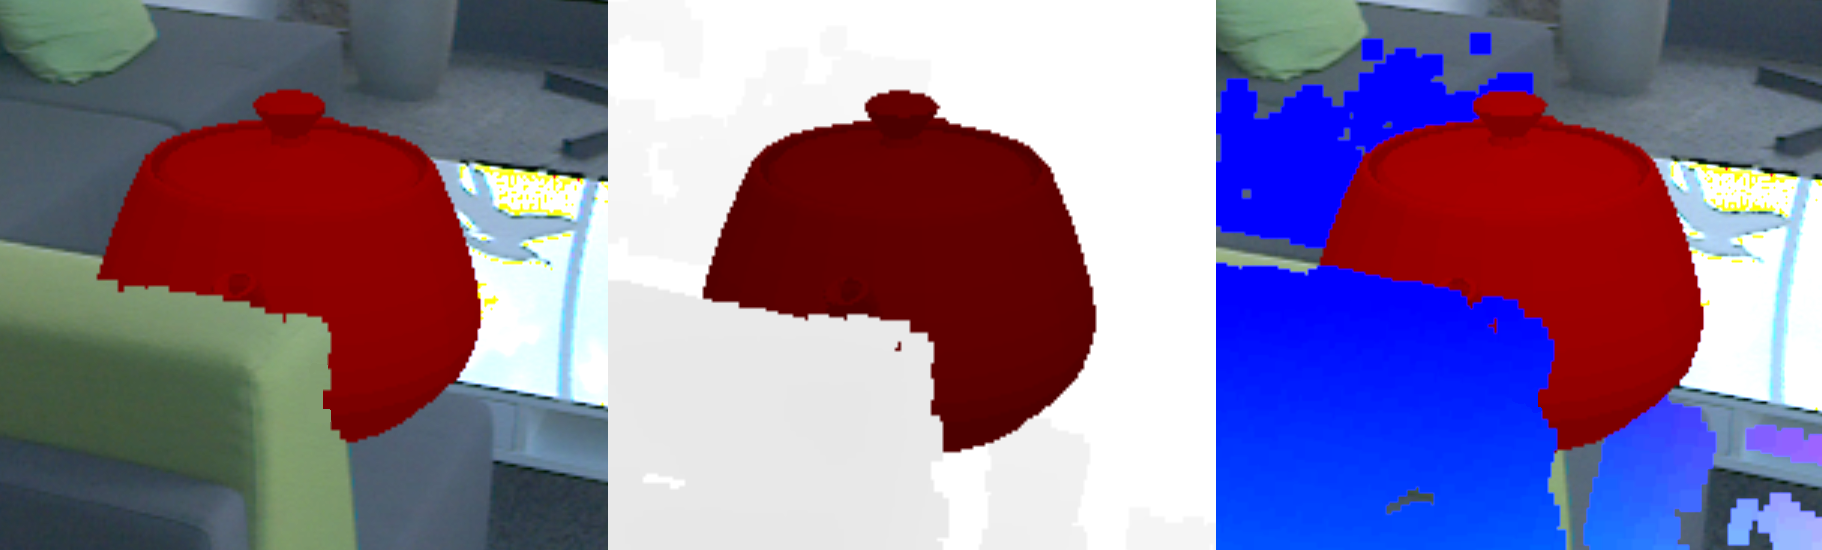
\includegraphics[width=1.0\textwidth]{content/images/methods/pc-noise.png} 
  \caption{Überdeckung mit einfacher Pointcloud Projektion. Links: Resultat der Überdeckung. Mitte: Darstellung des Tiefepuffers. Rechts: Darstellung der Pointcloud.}
  \label{fig:pc-noise}
\end{figure}

Die Reduktion von Ungenauigkeiten im Tiefenbild könnte durch einen Gaußschen Weichzeichner erreicht werden. Dieser würde jedoch die Kanten im Farbbild nicht berücksichtigen und somit fehlerhafte Tiefen Gradienten an den Kanten erzeugen. \citet{newcombe2011kinectfusion} wenden einen sogenannten \enquote{Bilateralen Filter} in ihrem KinectFusion System an, bevor sie die Tiefeninformationen in die TSDF Repräsentation einfließen lassen. Dieser Filter von \citet{tomasi1998bilateral} ermöglicht das Weichzeichnen ohne dabei die Kanten im Bild zu übergehen, bezieht sich jedoch nur auf das selbe Bild, auf dem der Filter angewendet wird. \\

\citet{liu2012guided} hingegen wenden einen sogenannten \enquote{Guided Filter} in Ihrem Verfahren zur Optimierung der der Tiefeninformationen für Kinect ähnliche Sensoren auf das Tiefenbild an. Dieser Filter von \citet{he2010guided} ist in der Lage, auf Grundlage eines anderen Leitbildes ein Weichzeichnen durchzuführen, ohne dabei die Kanten des Leitbildes zu überschreiten. Auch wenn \citet{petschnigg2004digital} eine Erweiterung, den Joint Bilateral Filter, vorstellen, der auf Basis eines anderen Leitbildes eine Weichzeichnung ohne Kantenüberschreitung ermöglicht, bietet der Guided Filter eine deutlich bessere Performance. Außerdem verhindert der Guided Filter Fehler Artefakte im Resultat, die bei dem Bilateralen Filter an den Kanten auftreten können. \citep{he2010guided} \\


Ausgehend von der Eingangsgrafik \(p\), einem Leitbild \(I\) und dem Ergebnisbild \(q\) wird das grundlegende lineare Modell des Guided Filter in der Gleichung \ref{eq:gf-model} beschrieben. Wobei \(w_k\) ein Ausschnitt von \(I\) um einen Pixel \(k\) ist und die beiden Koeffizienten \(a_k\) und \(b_k\) Konstanten im gegeben Ausschnitt sind, welche mit den Gelichungen \ref{eq:gf-a} und \ref{eq:gf-b} bestimmt werden können. \citep{he2010guided}


\begin{equation} \label{eq:gf-model}
q_{i} = a_{k} I_{i} + b_{k} , \forall i \in w_{k}
\end{equation}

\begin{equation} \label{eq:gf-a}
a_k = \frac{\frac{1}{w} \sum_{i \in w_k} I_i p_I - \mu_k \overline{p}_k}{\sigma_k^2+\epsilon}
\end{equation}

\begin{equation} \label{eq:gf-b}
b_k = \overline{p}_k - a_k\mu_k
\end{equation}

Die in den beschriebenen Koeffizienten-Gleichungen Variablen \(\mu_k\) und \(\sigma^2_k\) beschreiben jeweils den Mittelwert und die Abweichung des Leitbildes im Ausschnitt \(w_k\). Die Variable \(|w|\) entspricht dem festen Wert der Anzahl von Pixel im Ausschnitt \(w_k\). \(\overline{p}_k)\) ist wiederum der Mittelwert der Pixel im jeweiligen Ausschnitt, ermittelt durch \(\frac{1}{|w|}\sum_{i \in w_k} p_i\). Der Faktor \(\epsilon\) reguliert im beschriebenen Filter von \citet{he2010guided} welcher Ausschnitt als beizubehaltende Kante im resultierenden Bild gewertet werden soll. Neben diesem Regulierungsfaktor ist auch die Wahl des Radius \(r\) für den Ausschnitt \(w_k\) als Eingabe für diesen Filter wichtig. \citep{he2010guided} \\

\begin{figure}[h]
  \centering
	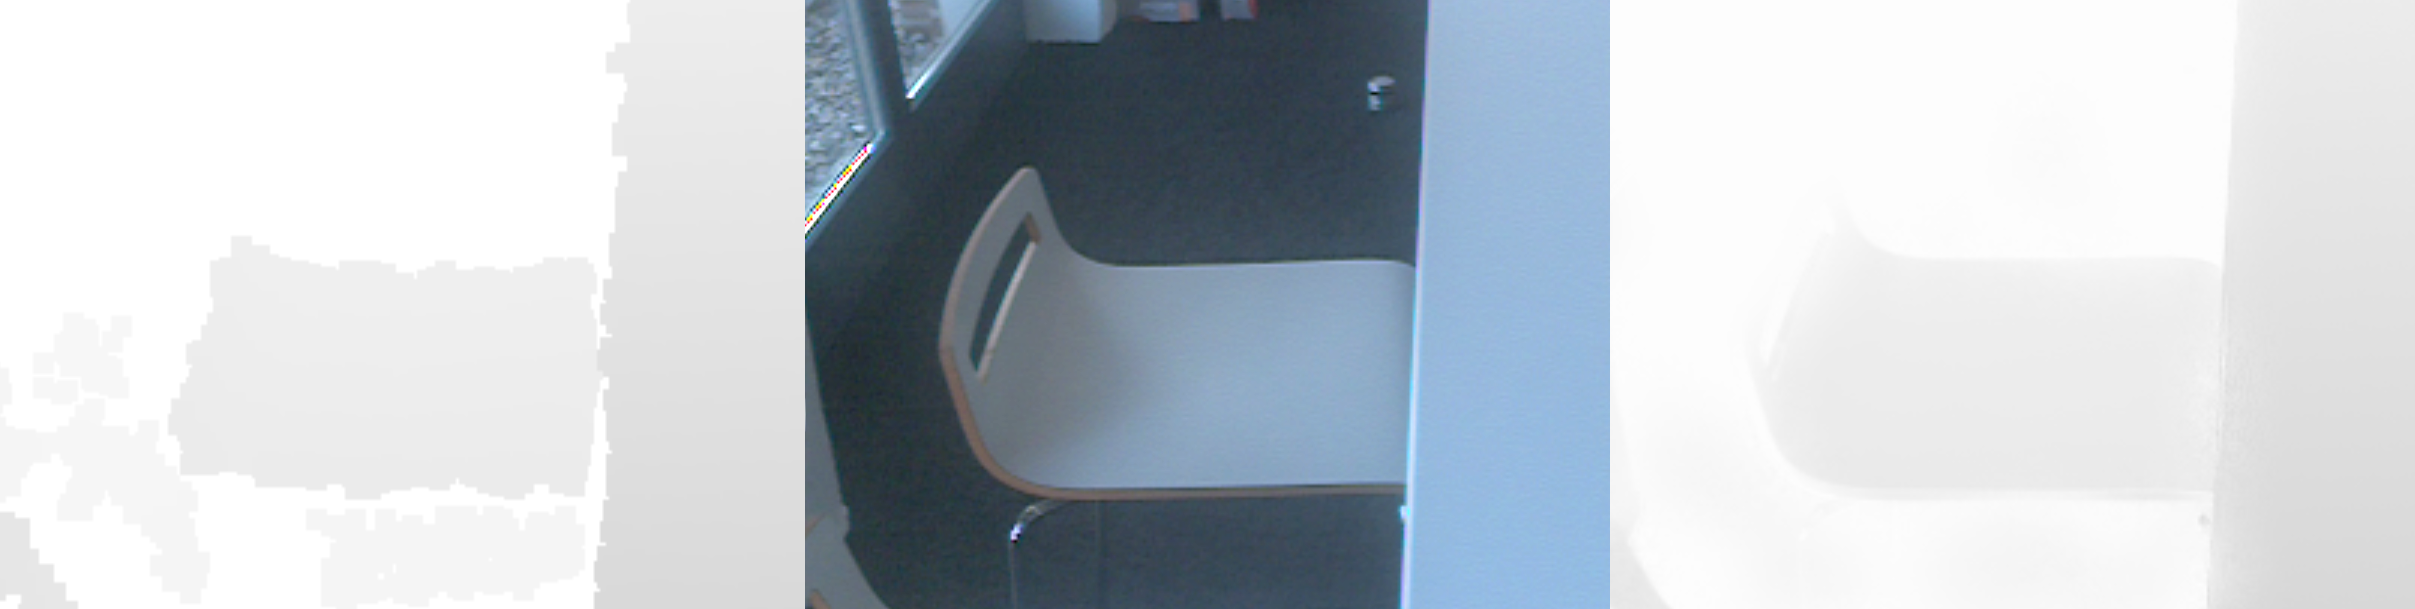
\includegraphics[width=1.0\textwidth]{content/images/methods/gf-result.png} 
  \caption{Guided Filter Anwendungsbeispiel. Das Tiefenbild links ergibt durch den Guided Filter mit dem Leitbild in der Mitte das Ergebnis im rechten Bild.}
  \label{fig:gf-result}
\end{figure}

Mit einer Komplexität von \(O(N)\) findet dieser Filter erfolgreich Anwendung  in verschiedensten Bereichen. Er wird zum Beispiel zur Rauschunterdrückung, dem Weichzeichnen oder Verstärken von Details, zur HDR Kompression, dem Entfernen von Matten Bildeigenschaften oder, wie in diesem Fall, zum zusammengeführten Anreichern von Bildinformationen verwendet \citep{he2010guided}. Angewendet auf das ermittelte Tiefenbild soll dieser Guided Filter, mit dem jeweiligen RGB Bild als Leitbild, ein Rauschen eliminieren und die Kanten der Tiefeninformationen, durch ein entsprechend groß gewählten Fensterradius \(r\) und Regulierungsfaktors \(\epsilon\), an die Kanten der Kameraaufnahme angleichen \citep{liu2012guided}. Ein Beispiel für eine erfolgreiche Anwendung dieses Filters ist in Abbildung \ref{fig:gf-result} zu sehen.


